\documentclass[pdftex,letterpaper,11pt]{article}
\usepackage[top=1in,bottom=1in,left=1in,right=1in]{geometry}

\usepackage[dvips]{graphicx}
\usepackage{amsmath}
\usepackage{amssymb}
\usepackage{color}
\usepackage[yyyymmdd]{datetime}
\usepackage{fancyhdr}
\usepackage{fancyvrb}
\usepackage[hidelinks]{hyperref}
\usepackage{pslatex}
\usepackage{algorithm}
\usepackage{algpseudocode}

\usepackage{subfig}
\usepackage{graphicx}
\usepackage[cache=false]{minted}

\usepackage{tikz, forest}
\usetikzlibrary{shapes.geometric}

\pagestyle{fancy}

\title{%
	It is the Champion \\
	\large Prototype findings}

\author{Jordan Aceto}

\setlength{\parindent}{0mm}
\setlength{\parskip}{2mm}

\lfoot{Jordan Aceto}
\cfoot{Page \thepage}
\rfoot{PDF: \today, \currenttime}

\renewcommand{\footrulewidth}{0.4pt}

\begin{document}

\maketitle

\tableofcontents

\newpage

\section{Basic Features}

\begin{itemize}
\item Single ended 6550 ouput stage, cathode biased.
\item Two 12AX7 tubes in the preamp.
\item Fairly high gain ``Trainwreck-ish'' preamp with four gain stages.
\item Conventional treble, middle, bass tone stack.
\item Gain and master volume controls.
\item Point to point wiring in a gutted Fender Vibro-Champ XD cabinet.
\item Power transformer: Hammond 276x.
\item Output transformer: Edcor GXSE15-8-3.5k
\item DC filaments for the first 12AX7, supplied by a separate Antek AN-0115 transformer.
\end{itemize}

\newpage

\section{Power Amp Details}

The single 6550 output tube was chosen to provide a little more ``oomph'' than a typical Champ-style single ended amp, but still be fairly low power for playing at home or in the studio at reasonable volumes.

\vspace{5mm}

\begin{figure}[H]
\centering
\caption{Power amp circuit}
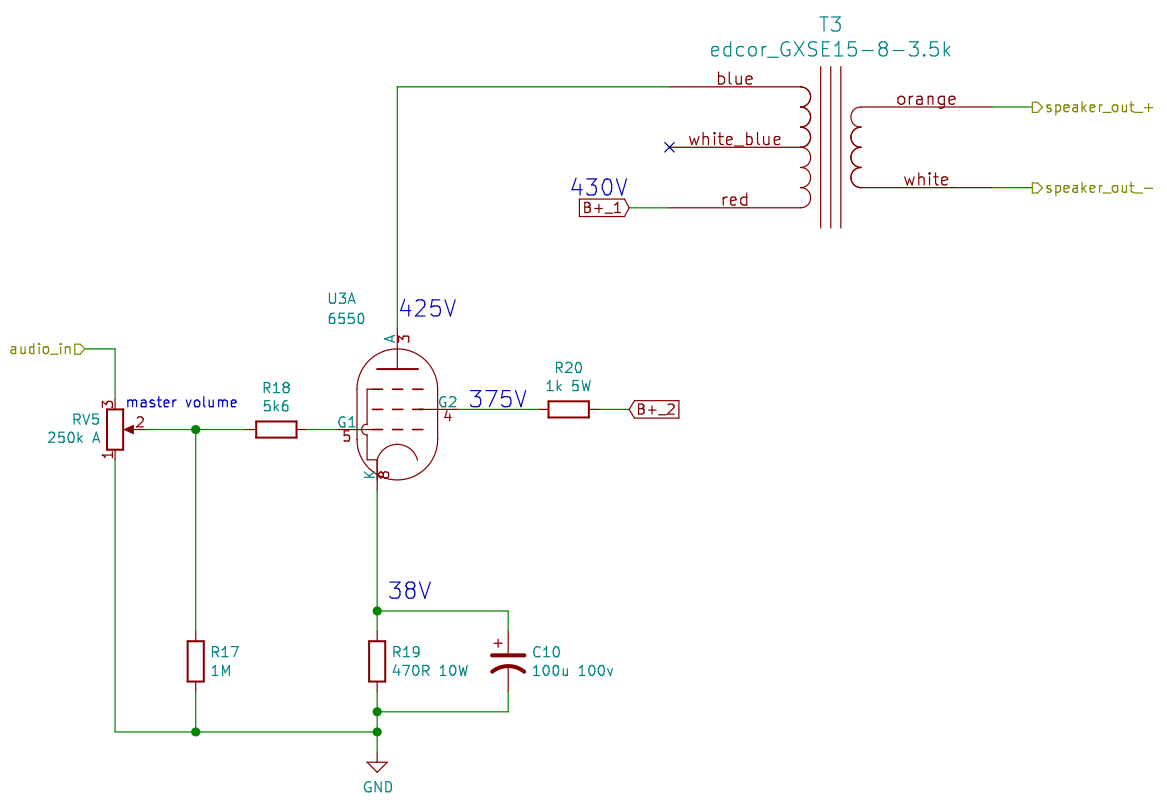
\includegraphics[width=.8\textwidth]{power_amp_circuit.png}
\end{figure}

As we can see by examining the voltage across the cathode resistor, about $80mA$ of bias current flows in the power tube at idle, for about 31 watts of dissipation. The maximum plate dissipation for this tube is 35 watts. I could probably bump up the bias a little bit, there is no compelling reason to do so for now.

\vspace{5mm}

After construction, the amp was hooked up to a dummy load to test the power output. The output transformer has a 438:1 turns ratio, and a variety of load resistances were tried out to experiment with the relationship between load impedance and power delivery. I have a big honkin' dummy load made up of a string of eight 2$\Omega$ resistors, and this allowed me to vary the load resistance, and thus the reflected primary impedance, by clipping heavy test leads across various resistors. The findings are summarized in the table below:

\begin{table}[H]
\centering
\begin{tabular}{ c | c | c }
    Load resistance  & Reflected impedance & Power out (Watts)  \\ \hline \hline
	4 & 1750 & 5.8 \\ \hline
	6 & 2628 & 8.5 \\ \hline
	8 & 3500 & 9.7 \\ \hline
	10 & 4380 & 10 \\ \hline
	12 & 5256 & 9.2 \\ \hline
	14 & 6132 & 8.8 \\ \hline
	16 & 7008 & 7.9 \\ \hline
\end{tabular}
\end{table}

The measured power output is an approximation and shouldn't be taken as a super precise measurement. I tried to adjust the signal to \textit{just} under the point of clipping while measuring the power output for each impedance, but this is a guitar amp and there is significant nonlinearity well below clipping. The exact point where ``clean signal'' stops and ``clipping'' begins is a fuzzy line, but I tried to at least keep things consistent between readings. 

\vspace{5mm}

The above table shows us that somewhere around 3.5k to 5k is a happy primary impedance for this circuit if we want to maximize power output. The chosen 3.5k$\Omega$ primary impedace seems just fine. A few fractions of a watt in either direction isn't going to bother anybody.

\vspace{5mm}

The distortion introduced by overdriving the power amp is quite pleasant, with a gradual introduction of compression, then crunch, then heavy distortion. This is illustrated in the oscilloscope shots below:

\vspace{5mm}

\begin{figure}[H]
    \centering
    \subfloat[\centering]{{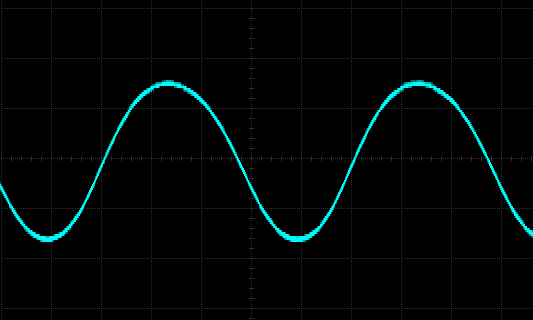
\includegraphics[width=.45\textwidth]{power_amp_scope_1.png} }}
    \qquad
    \subfloat[\centering]{{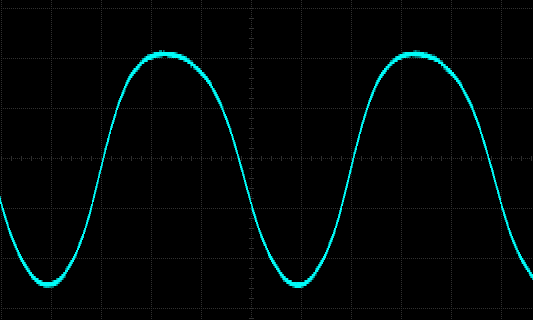
\includegraphics[width=.45\textwidth]{power_amp_scope_2.png} }}
    
    \subfloat[\centering]{{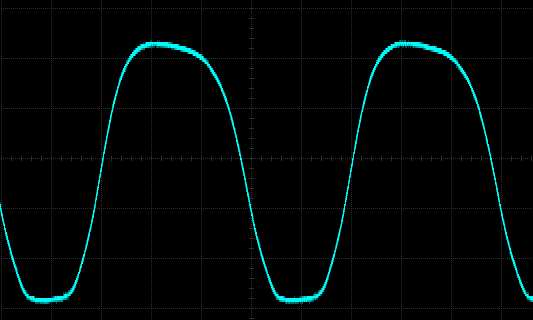
\includegraphics[width=.45\textwidth]{power_amp_scope_3.png} }}
    \qquad
    \subfloat[\centering]{{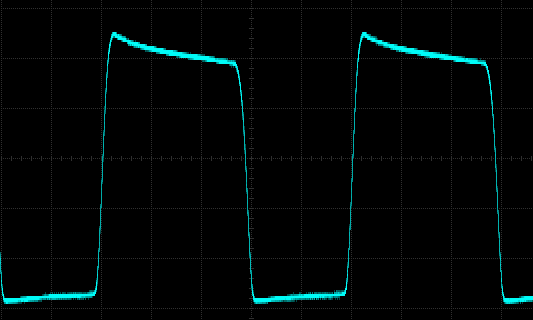
\includegraphics[width=.45\textwidth]{power_amp_scope_4.png} }}
\end{figure}

The asymmetric nature of the distortion may be partly due to the somewhat cold bias current. To me, the circuit sounds good and hits the desired output power, so there is little motivation to try to clean up the distortion or squeeze every last milliwatt out of it.

\end{document}